\documentclass[a4paper]{report}
\usepackage[utf8]{inputenc}
\usepackage[T1]{fontenc}
\usepackage{textcomp}

\usepackage{url}

\usepackage{hyperref}
\hypersetup{
    colorlinks,
    linkcolor={black},
    citecolor={black},
    urlcolor={blue!80!black}
}

\usepackage{graphicx}
\usepackage{wrapfig}
\usepackage{adjustbox}
\usepackage{float}
\usepackage[usenames,dvipsnames]{xcolor}

\usepackage{listings}

\lstset{
    language=Python,
    basicstyle=\ttfamily\footnotesize,
    keywordstyle=\color{blue},
    stringstyle=\color{red},
    commentstyle=\color{gray},
    showstringspaces=false,
    frame=single,
    numbers=left,
    numberstyle=\tiny,
    breaklines=true,
    tabsize=4
}

% \usepackage{cmbright}

\usepackage{amsmath, amsfonts, mathtools, amsthm, amssymb}
\usepackage{mathrsfs}
\usepackage{cancel}

\newcommand\N{\ensuremath{\mathbb{N}}}
\newcommand\R{\ensuremath{\mathbb{R}}}
\newcommand\Z{\ensuremath{\mathbb{Z}}}
\renewcommand\O{\ensuremath{\emptyset}}
\newcommand\Q{\ensuremath{\mathbb{Q}}}
\newcommand\C{\ensuremath{\mathbb{C}}}
\let\implies\Rightarrow
\let\impliedby\Leftarrow
\let\iff\Leftrightarrow
\let\epsilon\varepsilon

% horizontal rule
\newcommand\hr{
    \noindent\rule[0.5ex]{\linewidth}{0.5pt}
}

\usepackage{tikz}
% \usepackage{tikzmark}
\usepackage{pgfplots}
\usepackage{tikz-cd}

\usetikzlibrary{calc, arrows.meta, positioning, angles, quotes, patterns}

% theorems
\usepackage{thmtools}
\usepackage{thm-restate}
\usepackage[framemethod=TikZ]{mdframed}
\mdfsetup{skipabove=1em,skipbelow=0em, innertopmargin=12pt, innerbottommargin=8pt}

\theoremstyle{definition}

\makeatletter

\declaretheoremstyle[
    headfont=\bfseries\sffamily\color{ForestGreen!70!black}, bodyfont=\normalfont,
    mdframed={
        linewidth=2pt,
        rightline=false, topline=false, bottomline=false,
        linecolor=ForestGreen, backgroundcolor=ForestGreen!5,
    }
]{thmgreenbox}

\declaretheoremstyle[
    headfont=\bfseries\sffamily\color{NavyBlue!70!black}, bodyfont=\normalfont,
    mdframed={
        linewidth=2pt,
        rightline=false, topline=false, bottomline=false,
        linecolor=NavyBlue, backgroundcolor=NavyBlue!5,
    }
]{thmbluebox}

\declaretheoremstyle[
    headfont=\bfseries\sffamily\color{NavyBlue!70!black}, bodyfont=\normalfont,
    mdframed={
        linewidth=2pt,
        rightline=false, topline=false, bottomline=false,
        linecolor=NavyBlue
    }
]{thmblueline}

\declaretheoremstyle[
    headfont=\bfseries\sffamily\color{RawSienna!70!black}, bodyfont=\normalfont,
    mdframed={
        linewidth=2pt,
        rightline=false, topline=false, bottomline=false,
        linecolor=RawSienna, backgroundcolor=RawSienna!5,
    }
]{thmredbox}

\declaretheoremstyle[
    headfont=\bfseries\sffamily\color{RawSienna!70!black}, bodyfont=\normalfont,
    numbered=no,
    mdframed={
        linewidth=2pt,
        rightline=false, topline=false, bottomline=false,
        linecolor=RawSienna, backgroundcolor=RawSienna!1,
    },
    qed=\qedsymbol
]{thmproofbox}

\declaretheoremstyle[
    headfont=\bfseries\sffamily\color{NavyBlue!70!black}, bodyfont=\normalfont,
    numbered=no,
    mdframed={
        linewidth=2pt,
        rightline=false, topline=false, bottomline=false,
        linecolor=NavyBlue, backgroundcolor=NavyBlue!1,
    },
]{thmexplanationbox}

\declaretheorem[numberwithin=chapter, style=thmgreenbox, name=Definition]{definition}
\declaretheorem[sibling=definition, style=thmredbox, name=Corollary]{corollary}
\declaretheorem[sibling=definition, style=thmredbox, name=Proposition]{prop}
\declaretheorem[sibling=definition, style=thmredbox, name=Theorem]{theorem}
\declaretheorem[sibling=definition, style=thmredbox, name=Lemma]{lemma}
\declaretheorem[sibling=definition, style=thmbluebox,  name=Example]{eg}
\declaretheorem[sibling=definition, style=thmbluebox,  name=Nonexample]{noneg}
\declaretheorem[sibling=definition, style=thmblueline, name=Remark]{remark}




\declaretheorem[numbered=no, style=thmexplanationbox, name=Proof]{explanation}
\declaretheorem[numbered=no, style=thmproofbox, name=Proof]{preuve}
\declaretheorem[style=thmbluebox,  numbered=no, name=Exercise]{ex}
\declaretheorem[style=thmblueline, numbered=no, name=Note]{note}

% \renewenvironment{proof}[1][\proofname]{\begin{replacementproof}}{\end{replacementproof}}

% \AtEndEnvironment{eg}{\null\hfill$\diamond$}%

\newtheorem*{uovt}{UOVT}
\newtheorem*{notation}{Notation}
\newtheorem*{previouslyseen}{As previously seen}
\newtheorem*{problem}{Problem}
\newtheorem*{observe}{Observe}
\newtheorem*{property}{Property}
\newtheorem*{intuition}{Intuition}


\declaretheoremstyle[
    headfont=\bfseries\sffamily\color{RawSienna!70!black}, bodyfont=\normalfont,
    mdframed={
        linewidth=2pt,
        rightline=false, topline=false, bottomline=false,
        linecolor=RawSienna, backgroundcolor=RawSienna!5,
    }
]{todo}
\declaretheorem[numbered=no, style=todo, name=TODO]{TODO}


\usepackage{etoolbox}

\AtEndEnvironment{vb}{\null\hfill$\diamond$}%
\AtEndEnvironment{intermezzo}{\null\hfill$\diamond$}%




% http://tex.stackexchange.com/questions/22119/how-can-i-change-the-spacing-before-theorems-with-amsthm
% \def\thm@space@setup{%
%   \thm@preskip=\parskip \thm@postskip=0pt
% }

\usepackage{xifthen}

\def\testdateparts#1{\dateparts#1\relax}
\def\dateparts#1 #2 #3 #4 #5\relax{
    \marginpar{\small\textsf{\mbox{#1 #2 #3 #5}}}
}

\def\@lesson{}%
\newcommand{\lesson}[3]{
    \ifthenelse{\isempty{#3}}{%
        \def\@lesson{Lecture #1}%
    }{%
        \def\@lesson{Lecture #1: #3}%
    }%
    \subsection*{\@lesson}
    \testdateparts{#2}
}

% fancy headers
\usepackage{fancyhdr}
\pagestyle{fancy}

% \fancyhead[LE,RO]{Gilles Castel}
\fancyhead[RO,LE]{\@lesson}
\fancyhead[RE,LO]{}
\fancyfoot[LE,RO]{\thepage}
\fancyfoot[C]{\leftmark}
\renewcommand{\headrulewidth}{0pt}

\makeatother

% figure support (https://castel.dev/post/lecture-notes-2)
\usepackage{import}
\usepackage{xifthen}
\pdfminorversion=7
\usepackage{pdfpages}
\usepackage{transparent}
\usepackage[margin=0.8in]{geometry}
\newcommand{\incfig}[1]{%
    \def\svgwidth{\columnwidth}
    \import{./figures/}{#1.pdf_tex}
}

% %http://tex.stackexchange.com/questions/76273/multiple-pdfs-with-page-group-included-in-a-single-page-warning
\pdfsuppresswarningpagegroup=1
\pgfplotsset{compat=1.11}
\usepackage{subcaption}

\author{Yehor Korotenko}

\newcommand{\scalar}[2]{\langle #1, #2 \rangle}
\newcommand{\scalair}[1]{\left\langle #1 \right\rangle}

% fancy chapters
\usepackage{lipsum}
\usepackage[Lenny]{fncychap}
\ChNameUpperCase
\ChNumVar{\fontsize{40}{42}\usefont{OT1}{ptm}{m}{n}\selectfont}
\ChTitleVar{\Large\sc}



\title{Notes du cours d'Algebre Linéaire 2}


\begin{document}
\maketitle
\begin{abstract}
    Le cours parte sur deux sujets liées:
    \begin{enumerate}
        \item la théorie des espaces euclidiens (i.e un espace vectoriel réel muni d'un produit scalaire) et leur endomorphismes
        \item la réduction des endomorphismes d'un espace vectoriel de dimension finie
    \end{enumerate}
\end{abstract}

\chapter{Premier cours}
\section{Éspaces $\R^d$  $\C^d$}
\begin{definition}
    \[
        \R^d = \{ X = (x_1, \ldots, x_d), x_i \in \R\}
    \] 
    $x_1, \ldots, x_d$ coordonnées cartésiennes de X
\end{definition}
\begin{eg}
   $d = 2$ coordonnées polaires:  
   \begin{align*}
      &x = r \cos \theta \\
        & y = r \sin \theta\\
        &0 \le r \le  \infty \quad \theta \in [0, 2\pi[
   \end{align*}
   \begin{center}
       
\begin{tikzpicture}
    % Create the axis
    \begin{axis}[
        axis lines=middle,
        xmin=-1, xmax=3,
        ymin=-1, ymax=3,
        xlabel={$x$},
        ylabel={$y$},
        axis equal,
        height=6cm
    ]
        % Draw the vector
        \addplot[->, thick, blue] coordinates {(0,0) (3,2)} node[right] {$\vec{v}$};

        % Draw x-axis projection manually
        \draw[thick] (axis cs: 0,0) -- (axis cs: 3,0);

        % Use TikZ outside \addplot for \pic
        \node (A) at (2, 0) {};
        \node (C) at ($(0,0)!0.5!(3,2)$) {};
        \node (B) at (0, 0) {};
        \node[above] (_) at ($(0,0)!0.5!(3,2)$) {$r$};
        
        \pic [draw,-, black, angle eccentricity=1.2, angle radius=1cm,"$\theta$"] {angle = A--B--C};
    \end{axis}
\end{tikzpicture}
\end{center}
\end{eg}

\begin{definition}
    $\R^d$ est un espace vectoriel sur  $\R$ 
    \begin{align*}
        &\vec{X} + \vec{Y} = (x_1 + y_1, \ldots, x_d + y_d)\\
        &\lambda X = (\lambda x_1, \ldots, \lambda x_d) \quad \lambda \in \R\\
        &\vec{0}_d = \vec{0} = (0, \ldots, 0)
    \end{align*}
\end{definition}
\begin{definition}\label{def:prod_scalaire}
    Un \textbf{produit scalaire}:
    \[
    X \cdot Y = x_1y_1 + x_2y_2 + \ldots x_dy_d = \|X\|\|Y\|\cos(\theta) \text{ (où } \theta \text{ est une angle entre } X \text{ et } Y \text{)}
    \] 
\end{definition}
\begin{intuition}
    Ce produit nous dit \textit{how closely the vectors point in the same direction} (cosinus tend vers 1 quand $\theta$ tend vers 0º, et cosinus tend vers 0 quand  $\theta$ tend vers 90º). Et ce produit nous permet d'avoir une projection de $X$ sur $Y$ par la formule:
    \[
    Proj(X) = \frac{X \cdot Y}{\|Y\|} \cdot \frac{Y}{\|Y\|}
    \] 
    $X \cdot Y$ donne la longeur de  $X$ et  $Y$ ensemble, en divisant cette longeur par  $\|Y\|$ (la longeur de $Y$) on obtient la longeur de $X$ sur Y, il nous reste de multiplier cette longeur par un vecteur unitaire(de longeur 1) qui pointe dans la même direction que  $Y$, (on l'obtient par $\frac{Y}{\|Y\|}$)
   \begin{center}
      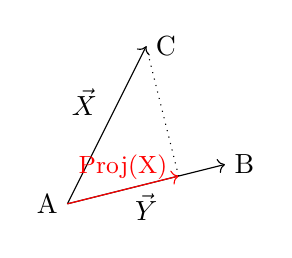
\begin{tikzpicture}
         \coordinate (A) at (0, 0); 
         \coordinate (B) at (2, 0.5);
         \coordinate (C) at (1, 2);
         \coordinate (newB) at (1.4117647059, 0.3529411765);
         \coordinate (dotBC) at (2, 1);
         \node[left] (_) at (A){A};
         \node[right] (_) at (B){B};
         \node[right] (_) at (C){C};
         \draw[->] (A) -- (B);
         \node[above left] (...) at ($(A)!0.5!(C)$) {$\vec{X}$};
         \node[below] (...) at ($(A)!0.5!(B)$) {$\vec{Y}$};
         \draw[->] (A) -- (C);
         \draw[->, red, thin] (A) -- (newB);
         \draw[dotted] (C) -- (newB);
         \node[above, red] (_) at ($(A)!0.5!(newB)$){\small Proj(X)};
      \end{tikzpicture} 
   \end{center}
\end{intuition}
\begin{prop}
    Produit scalaire respectes ces propriétés:
    \begin{enumerate}
        \item bilinaiarité $\quad \lambda \in \R$
            \begin{enumerate}
                \item $(X + Y) \cdot Z = X \cdot Z + Y \cdot Z$
                \item $(\lambda X) \cdot Z = \lambda (X \cdot Z)$
                \item $Z \cdot (X + Y) = Z \cdot X + Z \cdot Y$ 
                \item $Z \cdot (\lambda X) = \lambda (Z \cdot X)$
            \end{enumerate}
        \item symétrie $X \cdot Y = Y \cdot X$
        \item défini positif:  $X \cdot X \ge 0$ et $X \cdot X = 0 \iff X = 0_d$
    \end{enumerate}
\end{prop}
\begin{prop}
    \underline{Cauchy-Schwarz}:\\ 
    \[
        |X \cdot Y| \le (X \cdot X)^{\frac{1}{2}}(Y \cdot Y)^{\frac{1}{2}}
    \] 
\end{prop}
\begin{definition}\label{def:norm_eucl}
    La \textbf{norme euclidienne} d'un vecteur $X$ est noté:
   \[
       \|X\| = \left(\sum_{n=1}^{d} x_i^2\right)^{\frac{1}{2}} = \sqrt{x_1^2 + \ldots + x_d^2} = (X \cdot X)^{\frac{1}{2}}
   \] 
   souvent noté $\|X\|_2$
\end{definition}
\begin{intuition}
   Par le théorème de Pythogore, c'est une longeur de ce vecteur. 
\end{intuition}
\begin{prop}
    La norme suit ces propriétés:
   \begin{enumerate}
       \item $\|\lambda X\| = |\lambda|\|X\| \, X \in \R^d, \, \lambda \in \R$
       \item $\|X + Y\| \le \|X\| + \|Y\| \text{ (inégalité triangulaire)}$
       \item $\|X\| \ge 0$ et $\|X\| = 0 \iff X = 0_d$
   \end{enumerate}
\end{prop}
\begin{explanation}
    de (2)
    \begin{align*}
        \|X + Y\|^2 &= (X + Y)\cdot(X + Y) = X \cdot (X + Y) + Y \cdot (X + Y) = X \cdot X + X \cdot Y + Y \cdot X + Y \cdot Y\\
                    &= \|X\|^2 + 2X \cdot Y + \|Y\|^2 \le \|X\|^2 + 2\|X\| \|Y\| + \|Y\|^2 = (\|X\| + \|Y\|)^2
    \end{align*}
\end{explanation}
\begin{definition}
    Une \underline{norme} sur $\R^d$ est une application  $N: \: \R^d \to \R$ tell que:
    \begin{enumerate}
        \item $N(\lambda X) = |\lambda|N(X)$
        \item  $N(X + Y) \le N(X) + N(Y)$
        \item $N(X) \ge 0$ et $N(X) = 0 \iff X = 0_d$
    \end{enumerate}
\end{definition}
\begin{eg}
   \begin{align*}
       &\|X\|_1 = \sum_{n=1}^{d} |x_i|\\
       &\|X\|_{\infty} = \underset{1\le i \le n}{max} |x_i|
   \end{align*} 
\end{eg}
\section{Éspace $\C^d$}
\begin{definition}
    \[
        \C^d = \{ X = (x_1, \ldots, x_d): \: x_i \in \C\}
    \] 
    \begin{align*}
    &z \in \C \quad \overline{z} = a - ib \quad \overline{z}z = a^2 + b^2 \quad |z| = \sqrt{\overline{z}z} = \sqrt{a^2 + b^2}  \\
    &z = a + ib \qquad a = Re\,z,\,b = Im\,z\\
    &Re\,X = (Re\,x_1, \ldots, Re\,x_d) \in \R^d\\
    &Im\,X = (Im\,x_1, \ldots, Im\,x_d) \in \R^d\\
    &\underset{\in \C^d}{X} = \underset{\in \R^d}{Re\,X} + i\underset{\in \R^d}{\:Im\,X}\\
    \end{align*}
    $\C^d$ est un espace vécrotiel sur  $\C$ (même formules avec $\lambda \in \C$ corps des scalaires)
\end{definition}
\begin{definition}
    \underline{Produit scalaire:}
    \[
        (X|Y) = \sum_{n=1}^{d} \overline{x_i}y_i \in \C
    \] 
\end{definition}
\begin{prop}
   . 
   \begin{enumerate}
       \item $(X|Y)$ est "linéaire par rapport à Y"
           \begin{itemize}
               \item $(Z|X + Y) = (Z|X) + (Z|Y)$
               \item $(Z|\lambda X) = \lambda(Z|X) \quad \lambda \in \C$
               \item  $(Z|\lambda X + \mu Y) = \lambda(Z|X) + \mu(Z|Y)$
               \item  $(X + Y|Z) = (X|Z) + (Y|Z)$
               \item $(\lambda X|Z) = \overline{\lambda}(X|Z) \quad \lambda \in \C$
               \item $(\lambda X + \mu Y|Z) = \overline{\lambda}(X|Z) + \mu(Y|Z)$
           \end{itemize}
       \item $(Y|X) = \overline{(X|Y)}$
       \item $(X|X) = \sum_{n=1}^{d} \overline{x_i}x_i = \sum_{n=1}^{d} |x_i|^2$\\
           $(X|X) \ge 0$ et $(X|X) = 0 \iff X = 0_d$
   \end{enumerate}
\end{prop}
\begin{explanation}
    On a Cauchy-Schwarz:
    \begin{align*}
        (X|Y) \le (X|X)^{\frac{1}{2}}(Y|Y)^{\frac{1}{2}}
    \end{align*}
    même preuve qu'avant
\end{explanation}
On pose:
\begin{align*}
    \|X\| & \text{(ou }\|X\|_2\text{)}\\
          &= (X|X)^{\frac{1}{2}} = \left( \sum_{n=1}^{d} |x_i|^2 \right)^2
\end{align*}
norme hibertienne
\[
    \underset{\in \C^d}{\|X\|^2} = \underset{\in \R^d}{\|Re\,X\|^2} + i\underset{\in \R^d}{\:\|Im\,X\|^2}\\
\] 
\begin{lemma}
   \begin{align*}
       \|X\| = \underset{\|Y\|\le 1}{sup|(X|Y)|}
   \end{align*} 
\end{lemma}
\begin{explanation}
    $|(X|Y)| \le \|X\|\|Y\| \le \|X\|$ si $\|Y\| \le 1$
    \[
    \underset{\|Y\|\le 1}{sup|(X|Y)|}
    \] 
    \underline{Autre sens:} 
    \begin{align*}
        &X \neq 0 \quad Y =  \frac{X}{\|X\|} = \lambda X \quad \lambda = \frac{1}{\|X\|}\\
        &\|Y\| = |\lambda|\|X\| = \frac{1}{\|X\|}\|X\| = 1\\
        &(X|Y) = (X|\frac{X}{\|X\|}) = \frac{1}{\|X\|}(X|X) = \|X\|\\
        &sup \{|(X|Y)|: \, \|Y\| \le  1\}\\
        &\|X\| \le sup \{|(X|Y)|: \, \|Y\|\le 1\} \quad \text{(prendre }Y = \frac{X}{\|X\|}\text{)}
    \end{align*}

\end{explanation}
\underline{Autres normes sur $\C^d$}
\begin{itemize}
    \item $\|X\|_1 = \sum_{n=1}^{d} |x_i| \quad X \in \C^d$
    \item $\|X\|_{\infty} = \underset{1\le i \le d}{sup} |x_i|$
\end{itemize}
\section{Distance sur $\R^d$}
On oublie norme et produit scalaire. On introduit la distance
\begin{definition}\label{def:distance} La distance
    \[
        d(X, Y) = \|X - Y\| 
    \] 
\end{definition}
\begin{definition} La distance euclidienne
    \[
        d(X, Y) = \|X - Y\| = \sqrt{\sum_{n=1}^{d} (x_i - y_i)^2} 
    \] 
\end{definition}
\begin{prop}
    \begin{align*}
        d: \R^d &\longrightarrow \R \\
        (X, Y) &\longmapsto d((X, Y)) 
    .\end{align*}
    \begin{enumerate}
        \item $d(X, Y) = d(Y, X)$ (symétrie)
        \item $d(X, Y) \le d(X, Z) + d(Z, Y)$ (inég. triangulaire) $\forall X, Y, Z$ 
        \item $d(X, Y) \ge 0 \quad \forall X, Y$ et $d(X, Y) = 0 \iff X = Y$ 
    \end{enumerate}
\end{prop}
\begin{eg} Distances
   \begin{enumerate}
       \item $d_2(X, Y) = \|X - Y\|_2$ (distance euclidienne sur $\R^d$)
       \item $d_1(X, Y) = \|X - Y\|_1$\\
           $d_{\infty}(X, Y) = \|X - Y\|_{\infty}$
       \item distance logarithmique sur $\R_+$:  $d(a, b) = |b - a|$
           \[
               \log_{10}(a) = \frac{\log(a)}{\log(10)}
           \] 
           $x, y \in ]0, +\infty[$\\ 
           $d_{\log}(x, y) = |\log_{10}(\frac{y}{x})|$ \\
           $i$ est une distance sur  $]0, +\infty[$\\
           $d_{\log}(100, 110) = \log_{10}(1,1)$
       \item distance SNCF
           \begin{center}
               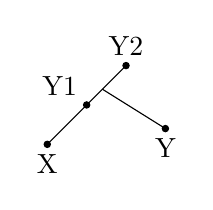
\begin{tikzpicture}
                  \coordinate (X) at (0, 0); 
                  \coordinate (Y) at (1.5, 0.2);
                  \coordinate (Y2) at (1, 1);
                  \coordinate (Y1) at ($(X)!0.5!(Y2)$);
                  \draw (X)--(Y2);
                  \draw (Y)--($(X)!0.7!(Y2)$);
                  \draw[fill=black] (X) circle (0.4mm);
                  \draw[fill=black] (Y) circle (0.4mm);
                  \draw[fill=black] (Y2) circle (0.4mm);
                  \draw[fill=black] (Y1) circle (0.4mm);
                  \node[below] (_) at (X){X};
                  \node[below] (_) at (Y){Y};
                  \node[above left] (_) at (Y1){Y1};
                  \node[above] (_) at (Y2){Y2};
               \end{tikzpicture}
               
           \end{center}
           $d(X, Y)$ distance usuelle dans  $\R^2$
           on pose:
            \begin{align*}
               \delta(X, Y) = \begin{cases}
                   d(X, Y) \text{ si } X, 0, Y \text{ alignés}\\
                   d(X, 0) + d(0, Y) \text{ sinon }
               \end{cases}
           \end{align*}
   \end{enumerate}
\end{eg}
\chapter{Éspaces métriques}
\begin{definition}
    $E$ muni d'une application de distance $d$ (voir Definition \ref{def:distance}) se note  $(E, d)$: \underline{espace métrique}
\end{definition}
\begin{remark}
   si $d_1 \neq d_2$ $(E, d_1)$ n'a rien à faire avec  $(E, d_2)$ 
\end{remark}
\begin{remark}
    Retenir la version suivante de l'inégalité triangulaire:
    \[
        |d(x, z) - d(y, z)| \le d(x, y)
    \] 
\end{remark}
\begin{remark}
    \underline{Distance induite:}\\
    Si $(E, d)$ espace métrique et  $U \subset E$. Je peux restreidnre $d$ à  $U \times U$:  $(U, d)$ est aussi un éspace metrique.
\end{remark}
\section{Boules dans un espace métrique}
\begin{definition}
    $(E, d)$ espace métrique. Soit  $x_0 \in E$ et $r \ge  0$
    \begin{enumerate}
        \item $B(x_0, r) = \{ x \in E: d(x_0, x) < r$ \} boule ouverte de centre $x_0$, de rayon $r$
        \item $B_f(x_0, r) = \{ x \in E: d(x_0, x) \le  r$\} boule fermée de centre $x_0$, de rayon $r$
    \end{enumerate}
\end{definition}
\begin{figure}
    \centering
    \begin{subfigure}{0.45\textwidth}
        \centering
        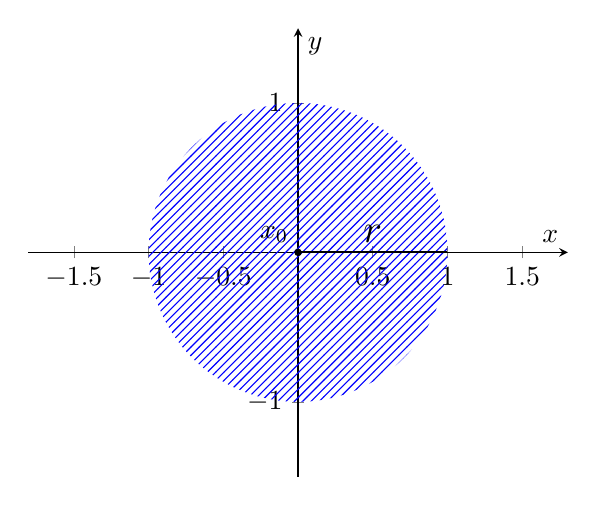
\begin{tikzpicture}
            \begin{axis}[
                axis equal, % Ensures the circle appears round
                axis lines=middle,
                xlabel={$x$},
                ylabel={$y$},
                xmin=-1.5, xmax=1.5,
                ymin=-1.5, ymax=1.5
                ]
                % Plot a circle with radius 1
                \addplot [
                    domain=0:360,       % Angle range
                    samples=200,        % Smoothness
                    fill=none,          % No solid fill color
                    pattern=north east lines, % Hatch pattern
                    pattern color=blue,
                    draw=none           % No outline
                    ] ({cos(x)}, {sin(x)}); 
                \node[above left] (_) at (0, 0){$x_0$};
                \draw[fill=black] (0, 0) circle (0.4mm);
                \draw[thick] (0,0)--(1,0);
                \node[above] (r) at ($(0,0)!0.5!(1,0)$){\Large$r$};
            \end{axis}
        \end{tikzpicture}
        \caption{boules ouverte (i.e $d(x_0, x) < r$)}
    \end{subfigure}
    \hfill
    \centering
    \begin{subfigure}{0.45\textwidth}
        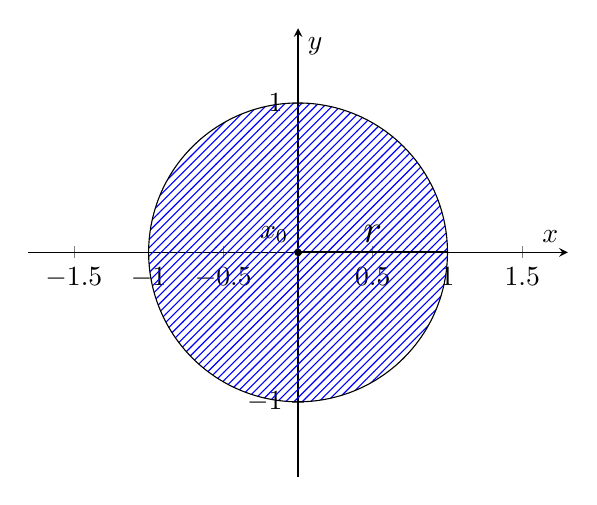
\begin{tikzpicture}
            \begin{axis}[
                axis equal, % Ensures the circle appears round
                axis lines=middle,
                xlabel={$x$},
                ylabel={$y$},
                xmin=-1.5, xmax=1.5,
                ymin=-1.5, ymax=1.5
                ]
                % Plot a circle with radius 1
                \addplot [
                    domain=0:360,       % Angle range
                    samples=200,        % Smoothness
                    fill=none,          % No solid fill color
                    pattern=north east lines, % Hatch pattern
                    pattern color=blue,
                    ] ({cos(x)}, {sin(x)}); 
                \node[above left] (_) at (0, 0){$x_0$};
                \draw[fill=black] (0, 0) circle (0.4mm);
                \draw[thick] (0,0)--(1,0);
                \node[above] (r) at ($(0,0)!0.5!(1,0)$){\Large$r$};
            \end{axis}
        \end{tikzpicture}
        \caption{boules fermée (i.e $d(x_0, x) \le r$)}
    \end{subfigure}
\end{figure}
\begin{lemma}.
   \begin{enumerate}
       \item $B(x_0, 0) = \O$ (car impossible d'avoir des points qui en distance sont strictement plus petit que 0)
       \item $B_f(x_0, 0) = \{x_0\}$
       \item $B(x_0, r_1) \subset B_f(x_0, r_1) \subset B(x_0, r_2)$ si $r_1 < r_2$
       \item $B(x_1, r_1) \subset B(x_0, r)$ si  $d(x_0, x_1) + r_1 \le r$
   \end{enumerate} 
   pic 5
\end{lemma}
\begin{explanation}
   Je suppose que $d(x_0, x_1) \le r$\\ 
   Soit $x \in B(x_1, r_1)$ donc $d(x_1, x) < r_1$ à montrer: $x \in B(x_0, r)$ (i.e $d(x_0, x) < r$?)\\
   L'inégalité triangulaire me dit:
   \begin{align*}
       d(x_0, x) &\le d(x_0, x_1) + d(x_1, x)\\
                 &< d(x_0, x_1) + r_1 \le r\\
                 &\implies x \in B(x_0, r)
   \end{align*}
\end{explanation}

\section{Bases orthonormales}
Soit $(E, \scalair{,})$ un espace euclidien et  $F \subset E$ un sous-espace vectoriel ($dim(F) < \infty$) car $dim(E) < \infty$.
\begin{note}
    \[
        F^{\perp} := \{x \in E \mid \scalair{X, Z} = 0 \, \forall z \in F\} 
    \] 
    l'orthogonale de $F$.
\end{note}
\begin{theorem}
    On a $E = F \oplus F^{\perp}$.\\
    En particulier,  $dim(F^{\perp}) = dim(E) - dim(F)$ et  $F = (F^{\perp})^{\perp}$
\end{theorem}
\begin{preuve}
   On doit montrer que:
   \begin{enumerate}
       \item $F \cap F^{\perp} = \O$
       \item $E = F + F^{\perp}$ i.e  $\forall x \in E, \exists x' \in F, \, x'' \in F^{\perp}$ tq $x = x' + x''$ 
   \end{enumerate}
   \begin{enumerate}
       \item Soit $x \in F \cap F^{\perp}$\\
       $\implies$ $\scalair{X, Z} = 0 \, \forall Z \in F$ car $x \in F \implies \scalair{X, X} = 0 \implies x = 0 (\scalair{,} \text{ est définie})$ 
        \item Soit $x \in E$. Considérons  $f_x \in E^{*}$, i.e  $f_x: E \to \R, y \mapsto \scalair{x, y}$ et $f := f_{x|F}: F \to \R \implies f \in E^{*}$
            Lemme de Riesz $\implies$ $\exists! x' \in F$ tq $f = f_{x'}: F \to \R, z \mapsto \scalair{x', z}$\\
            $\implies f_{x}(z) = f_{x'}(z) = f(z)\, \forall z \in F$ (Attention: pas l'égalité pour tout $z$ dans  $E$)\\
            Posons $x'' := x - x'$, i.e  $x = x' + x'' \in F$. Montrons  $x'' \in  F^{\perp}$.\\
            Si $z \in F$,  $\scalair{x'', z} = \scalair{x - x', z} = \scalair{x, z} - \scalair{x', z} = 0$. Donc $x'' \in F^{\perp}$ et  $E = F \oplus F^{\perp}$ ($dim(E) = dim(F) + dim(F^{\perp})$) \\
            $F \subseteq (F^{\perp})^{\perp}$ car $\scalair{x, z} = 0 \, \forall x \in F \, \forall z \in F^{\perp}$
            \[
                dim(F) = dim(E) - dim(F^{\perp})
            \] 
            car $E = G \oplus G^{\perp}$, donc  $dim(G) = dim(E) - dim(G^{\perp})$ pour  $G = F^{\perp}, \, dim(F^{\perp}) = dim(G)$
   \end{enumerate}
\end{preuve}
\begin{definition}
    Soit $E$ un espace vectoriel muni d'un produit scalaire  $\scalair{,}$
     \begin{itemize}
         \item Une famille $(v_i)_{i \ge 0}$ de vecteurs de $E$ est dite \underline{orthogonale} si pour $i \neq j$ on a $\scalair{v_i, v_j} = 0$ i.e  $v_i \perp v_j$
         \item Une famille orthonormale de  $E$ est une famille orthogonale  $(v_i)_{i \ge  0}$ tq de plus $\|v_i\| = 1$ pour  $i \ge 0$
    \end{itemize}
\end{definition}
\begin{eg}
   \begin{enumerate}
       \item $E = \R^{n}$ muni du produit scalaire canonique. La base canonique $(e_1, \ldots, e_n)$ est orthogonale car 
           \[
           \scalair{e_i, e_j} = \begin{cases}
               1 \text{ si } i = j\\
               0 \text{ si } i \neq j
           \end{cases}
           \] 
       \item Dans $E = \mathcal{C}^{0}([-1, 1], \R)$ muni de $\scalair{f,g} = \int_{-1}^{1} f(t)g(t)\,d{t}$. La famille $(\cos(t), \sin(t))$ est orthogonale. La famille $(1, t^2)$ n'est pas orthogonale:
            \[
                \scalair{1, t^2} = \int_{-1}^{1} 1 t^2 \, d{t} = \frac{2}{3} \neq  0 
           \] 
   \end{enumerate} 
\end{eg}
\begin{prop}
    Une famille orthogonale constituée de vecteurs \underline{non-nuls} est libre. En particulier, une famille orthonormale est libre. 
\end{prop}
\begin{preuve}
    Suppososns $(v_1, \ldots, v_n)$ orthogonale avec $v_i \neq 0 \, \forall i = 1, \ldots, n$\\
    si $\sum_{j=1}^{n} \underset{\in \R}{\alpha_iv_i} = 0$, alors  
    \[
        \forall i \in \{1, \ldots, n\} 0 = \scalair{v_i, \sum_{j=1}^{n} \alpha_jv_j} = \sum_{j=1}^{n}\alpha_j \scalair{v_i, v_j} = \alpha_i \underset{\neq 0}{\|v_i\|^2}
    \] 
    Donc $\alpha_i = 0 \, \forall i = 1, \ldots, n$.\\
    Si $(v_1, \ldots, v_n)$ est orthonormale, alors $\|v_i\| = 1$. Donc  $v_i \neq 0, \, \forall i = 1, \ldots, n$.
\end{preuve}
\begin{intuition}
   Les vecteurs orthogonales (perpendiculaires) ne sont jamais dans l'un l'autre (i.e $e_i = \lambda e_j$ n'est pas possible) si les vecteurs sont liés, soit l'angle est $< 90º$ (donc les vecteurs ne sont pas orthogonales, absurd), (ils sont dans l'un l'autre, ils ne sont pas orthogonales, absurd). Donc ils sont bien libres.
\end{intuition}
\begin{definition}
    $(E, \scalair{,})$ espace euclidien. Une famille  $B = (e_1, \ldots, e_n)$ est une base orthonormale (où BON) si elle est une base et famille orthonormale.
\end{definition}
\begin{theorem}
    $(E, \scalair{,})$ espace euclidien. Alors, il admet une BON.
\end{theorem}
\begin{preuve}
   Soit $n := dim(E)$. Soit  $(e_1, \ldots, e_p)$ une famille orthogonale (du point de vue du cardinal $p$) tq  $e_i \neq 0 \, \forall i = 1, \ldots, p$.\\
Supposons par l'absurde que $p < n$. Posons  $F = Vect(e_1, \ldots, e_p)$. Alors, $E = F \oplus F^{\perp}$ et  $dim(F) \le p < n$. Donc $F^{\perp} \neq  \{0\}$. Soit $x \in F^{\perp}, \, x \neq 0$. Alors, $(e_1, \ldots, e_p, x)$ est orthogonale de cardinale $> p$. Donc,  $p = n$ et  $(e_1, \ldots, e_n)$ est une base de $E$. Pour avoir une famille orthonormale  $(e_1', \ldots, e_n')$ il suffit de prendre $e_i' = \frac{1}{\|e_i\|}e_i \, \forall i = \{1, \ldots, n\}$.
\end{preuve}
\begin{prop}
    Soit $(E, \scalar{}{})$ un espace euclidien et soit  $(e_1, \ldots, e_n)$ une BON de $E$. Si  $x \in E$, on a:
   \[
       x = \sum_{i=1}^{n} \scalar{x}{e_i}e_i
   \] 
Autrement dit, le réél $\scalar{x}{e_i}$ est la  $i^{\text{ème}}$ coordonnée de $x$ dans la base  $(e_1, \ldots, e_n)$.
\end{prop}
\begin{intuition}
    L'orthonormalité de la base nous simplifie la vie. Mais avant, petite introduction. Soit un e.v $E = \R^2$ et la base $(e_1, e_2) = (\begin{pmatrix} 1 \\ 0 \end{pmatrix}, \begin{pmatrix} 0\\ 1 \end{pmatrix})$. Soit un vecteur $\vec{v} = (2, 3)$ :
    \begin{center}
        \begin{tikzpicture}
            \begin{axis}[
                scale=1,
                axis lines=middle,        % Draw axes in the middle
                xmin=-2, xmax=4,          % X-axis range
                ymin=-2, ymax=4,          % Y-axis range
                xlabel={$x$},             % Label for X-axis
                ylabel={$y$},             % Label for Y-axis
                xtick={-2,-1,0,1,2,3,4},% X-axis ticks
                ytick={-2,-1,0,1,2,3,4},% Y-axis ticks
                ]
            \draw[color=red, ->, thick] (0, 0) -- node[below]{$e_1$}(1, 0);
            \draw[color=blue, ->, thick] (0, 0) -- node[left]{$e_2$}(0, 1);
            \draw[color=green, ->] (0, 0) --node[above]{$\vec{v}$} (2, 3);

            \draw[color=gray, ->, thick] (1, 0) -- node[below]{$e_1$}(2, 0);
            \draw[color=gray, ->, thick] (2, 0) -- node[left]{$e_2$}(2, 1);
            \draw[color=gray, ->, thick] (2, 1) -- node[left]{$e_2$}(2, 2);
            \draw[color=gray, ->, thick] (2, 2) -- node[left]{$e_2$}(2, 3);

            \node[right, above] (_) at (2, 3){$(2, 3)$};
        \end{axis} 
        \end{tikzpicture}
    \end{center}
    Donc, on peut écrire $\vec{v} = \vec{(2, 3)} = 2 \cdot \vec{e_1} + 3 \cdot \vec{e_2}$. Les $x$ et  $y$ (les coordonnées de $v$) nous donnes combien de parties de chaque vecteur de bases (le nombre peut être $\in \R$) et prendre leurs sommes, pour obtenir $\vec{v}$. (Le plus simple: combien on doit aller à gauche et en haut).
    \par
    Dans la base orthonormale $\scalair{v, e_i}$ nous donne combien on prend d'un vecteur $e_i$ pour faire le vecteur  $\vec{v}$ et  $\vec{e_i}$ donne la direction. D'où $\scalair{v, e_1}$ équivaut à $2$, et  $\scalair{v, e_2}$ à  $3$, puis: 
   \[
       \vec{v} = \underbrace{\scalair{v, e_1}}_{= 2} \cdot \vec{e_1} + \underbrace{\scalair{v, e_2}}_{= 3} \cdot \vec{e_2}
   \]  
   Habituelement, pour trouver les coordonnées dans une base, on devrait résoudre un système linéaire, tandis qu’une base orthonormale permet de les obtenir en calculant le produit scalaire avec chaque vecteur de la base, ce qui est beaucoup plus simple.
\end{intuition}
\begin{preuve}
    Posons $y := \sum_{i=1}^{n} \scalar{x}{e_i}e_i$ . Alors, 
   \begin{align*}
       &\forall j = 1, \ldots, n,\\
       &\scalar{x - y}{e_j}\\ 
       = &\scalar{x}{e_j} - \scalar{y}{e_j}\\ 
       = &\scalar{x}{e_j} - \scalar{\sum_{i=1}^{n} \scalar{x}{e_i}e_i}{e_j}\\ 
       = &\scalar{x}{e_j} - \underbrace{ \sum_{i=1}^{n} \scalar{x}{e_i} }_{\substack{\text{moved out}\\ \text{like constant}}}\scalar{e_i}{e_j}\\ 
       = &\scalar{x}{e_j}\\ 
       -& \left(\scalar{x}{e_1}\underbrace{ \scalar{e_1}{e_j} }_{= 0} + \ldots + \scalar{x}{e_{j-1}}\underbrace{\scalar{e_{j-1}}{e_j}}_{= 0} + \scalar{x}{e_{j}}\underbrace{ \scalar{e_{j}}{e_j} }_{= 1} + \scalar{x}{e_{j+1}}\underbrace{ \scalar{e_{j+1}}{e_j} }_{= 0} + \ldots + \scalar{x}{e_{n}}\underbrace{ \scalar{e_{n}}{e_j} }_{= 0}\right)\\
        &\text{(} \forall i \neq j, \, \scalar{e_i}{e_j} = 0 \text{ car un produit scalaire des vecteur orthogonaux)}\\ 
        &\text{(} \forall j \, \scalar{e_j}{e_j} = 1 \text{ car un produit scalaire de même vecteur)}\\
       = &\scalar{x}{e_j} - \scalar{x}{e_j}\underset{= 1}{\scalar{e_j}{e_j}} = 0
   \end{align*}
   Donc, $x - y \in Vect(e_1, \ldots, e_n)^{\perp} = E^{\perp} = \{0\}$. Donc $x = y$
\end{preuve}
\begin{corollary}
    $\forall x \in E, \, \|x\|^2 = \sum_{i=1}^{n} \scalar{x}{e_i}^2$ 
\end{corollary}
\begin{preuve}
    Si $x = \sum_{i=1}^{n} \scalar{x}{e_i}e_i = \sum_{i=1}^{n} x_ie_i$ donc
    \[
        \|x\|^2 = \scalar{\sum_{i=1}^{n} x_ie_i}{\sum_{j=1}^{n} x_je_j} = \sum_{i,j=1}^{n} x_ix_j\scalar{e_i}{e_j} = \sum_{i=1}^{n} x_i^2
    \] 
\end{preuve}
\section{Matrices et produits scalaires}
\begin{prop} Soient $(E, \scalair{,})$ un espace euclidien et $\epsilon = (e_1, \ldots, e_n)$ une BON. Soient $f \in \mathcal{L}(E, E)$ et $A = (a_{i,j})_{1 \le i,j \le n}$ la matrice représentative de $f$ dans  $\epsilon$, i.e,  $A = Mat_{\epsilon}(f)$ 
    \[
        a_{i,j} = \scalair{f(e_i), e_j} \, \forall i,j = 1, \ldots, n
    \] 
\end{prop}
\begin{preuve}
   $A$ est la matrice dont les colonnes sont les vecteurs  $f(e_j)$ écrits dans la base $\epsilon$:
    \[
        A = (f(e_1) | \ldots | f(e_n))\quad f(e_j) = \begin{pmatrix} a_{1,j}\\ \ldots\\ a_{n, j} \end{pmatrix} 
   \] 
   Car $\forall v \in E, \, v = c_1e_1 + \ldots c_ne_n$ donc $f(v) = c_1f(e_1) + \ldots c_nf(e_n)$ par la linéarité, donc il nous reste à étudier chaque $f(e_j)$
   \begin{align*}
       f(e_j) = a_{1, j}e_1 + \ldots a_{n, j}e_n \implies\\
       \langle f(e_j), e_i \rangle = \left\langle \sum_{k=1}^n a_{k,j} e_k, e_i \right\rangle = \sum_{k=1}^{n} a_{k,j}\scalar{e_k}{e_i} = a_{k, j}
   \end{align*}
   car $\scalar{e_k}{e_j} = \begin{cases}
       0 \text{ si } k \neq j\\
       1 \text{ si } k = j
   \end{cases}$
   Donc:
   \[
       a_{i, j} = \scalair{f(e_j), e_i}
   \] 
\end{preuve}


La matrice d'un produit vectoriel est très utile dans l'algèbre linéaire. Avant donner une definition:
\par
Soit $E$ un espace vectoriel de dimension finie  $n$, un espace  $K$ et une forme bilinéaire  $b: E \times E \longrightarrow K$. Si $\{e_1, \ldots, e_n\}$ est une base de $E$, alors:  $x = \sum_{i=1}^{n} x_ie_i$ et $y = \sum_{j=1}^{n} y_je_j$, alors on a:
\[
b(x, y) = \sum_{i,j = 1}^{n} x_iy_jb(e_i, e_j)
\] 
$b$ est donc détérminé par la conaissance des valeurs  $b(e_i, e_j)$ sur une base.
 \begin{definition}
     On appelle  \textbf{matrice de $b$} dans la base $\{e_i\}$ la matrice:
      \[
          M(b)_{e_i} = \begin{pmatrix} 
              b(e_1, e_1) & b(e_1, e_2) & \ldots & b(e_1, e_n)\\
              b(e_2, e_1) & b(e_2, e_2) & \ldots & b(e_2, e_n)\\
              \ldots & \ldots & \ldots & \ldots\\
              b(e_n, e_1) & \ldots & \ldots & b(e_n, e_n)
          \end{pmatrix} 
     \] 
     Ainsi l'élément de la $\text{i}^{\text{ème}}$ ligne et $\text{j}^{\text{ème}}$ colonne est le coefficient de $x_iy_j$.
\end{definition}
\begin{eg}
   La matrice du produit scalair canonique dans $\R^3$ est:
   \[
       \scalair{X, Y} = x_1y_1 + x_2y_2 + x_3y_3 
   \] 
   \[
       Mat(\scalair{,})_{e_i} = \begin{pmatrix} 
            1 & 0 & 0\\
            0 & 1 & 0\\
            0 & 0 & 1
       \end{pmatrix} 
   \] 
\end{eg}
\begin{prop}\label{prop:prod-scal-par-matrice} produit scalair représenté par une matrice.\par
   Notons:
   \begin{align*}
       \underbrace{A = M(b)_{e_i}}_{\text{matrice de produit scalair}} && \underbrace{X = M(x)_{e_i}}_{\substack{\text{coordonnées de $x$}\\ \text{dans la base  $e_i$}}} && \underbrace{Y = M(y)_{e_i}}_{\substack{\text{coordonnées de $y$}\\ \text{dans la base $e_i$}}} && (x, y \in E)
   \end{align*}
   Alors, on a:
   \[
       b(x, y) = X^{t}AY
   \] 
\end{prop}
\begin{eg}
    Repronnons l'exemple avec $b = \scalair{,}$ le produit scalair canonique dans  $\R^3$. Soit $X = \begin{pmatrix} 1 \\ 2 \\ -1 \end{pmatrix}$ et $Y = \begin{pmatrix} 2 \\ 3 \\ 1 \end{pmatrix} $ dans la base canonique de $\R^3$. Donc:
    \begin{align*}
        \scalair{x, y} = X^{t}AY &= \overbrace{(1, 2, -1)}^{X^{t}} \times \overbrace{\begin{pmatrix} 1 & 0 & 0\\ 0 & 1 & 0\\ 0 & 0 & 1 \end{pmatrix}}^{A} \times \overbrace{ \begin{pmatrix} 2 \\ 3 \\ 1 \end{pmatrix} }^{Y} \\
                                 &= \underbrace{(1, 2, -1)}_{X} \times \underbrace{ \begin{pmatrix} 2 \\ 3\\ 1 \end{pmatrix} }_{A \times Y} \\
                                 &= 1 \cdot 2 + 2 \cdot 3 + (-1) \cdot 1 = 2 + 6 - 1 = 7
    \end{align*}
\end{eg}
\begin{TODO}
   changement de base de la matrice d'une forme bilinéaire 
\end{TODO}

\section{Projections orthogonales}
Soit $(E, \scalair{,})$ un espace euclidien,  $F \subseteq E$ un sous-espace vectoriel. Alors,  $E = F \oplus F^{\perp}$. Donc $\forall x \in E$ s'ecrit 
\[
x = \underset{\in F}{x_F} + \underset{\in F^{\perp}}{x_{F^{\perp}}}
\] 
\begin{definition}
    La \textbf{projection orthogonale} de $E$ dans  $F$ est la projection  $p_F$ de  $E$ sur  $F$ parallèlement  à $F^{\perp}$, i.e
    \begin{align*}
        p_F: E = F \oplus F^{\perp} &\longrightarrow F \\
        x = x_F + x_{F^{\perp}} &\longmapsto p_F(x = x_F + x_{F^{\perp}}) = x_F
    .\end{align*}
\end{definition}
\begin{remark}
   \begin{enumerate}
       \item $p_F$ est linéaire
       \item  $\forall x \in E \, p_{F}(x)$ est complétement caractérisé par la propriété suivante:\\
           Soit $y \in E$, alors
            \[
                y = p_F(x) \iff \left( \underset{\implies y = x_F}{y \in F \text{ et } x - y} \in F^{\perp} \right) 
           \] 
       En particulier $\scalair{p_F(x), x - p_F(x)} \,= 0$. Alors, si $(v_1, \ldots, v_R)$ est une BON de $F$, on a:
            \[
                \forall x \in E, \, p_F(x) = \sum_{i=1}^{k} \scalair{x, v_i}v_i
           \] 
           En effet, il suffit de vérfier que le vecteur $y = \sum_{i=1}^{k} \scalair{x, v_i}v_i$ vérfie:
           \[
               y \in F \text{ et } x - y \in F^{\perp}
           \] 
   \end{enumerate} 
\end{remark}
\begin{figure}[H]
   \centering 
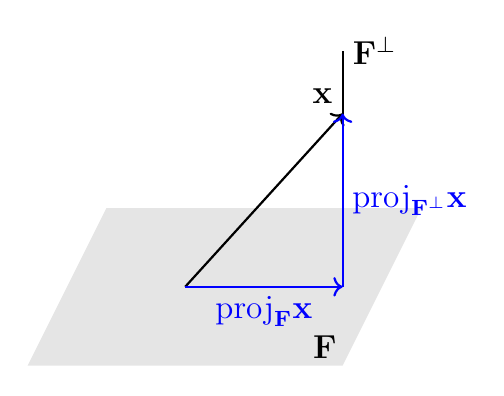
\begin{tikzpicture}

% Draw the plane
\fill[gray!20] (-2,-1) -- (2,-1) -- (3,1) -- (-1,1) -- cycle;

% Draw the vectors
\draw[->, thick, black] (0,0) -- (2,2.2) node[anchor=south east] {\large $\mathbf{x}$};

\node[anchor=north, blue] (_) at ($(0,0)!0.5!(2,0)$) {\large $\text{proj}_\mathbf{F} \mathbf{x}$};
\node[anchor=west, blue] (_) at ($(2,0)!0.5!(2,2.2)$) {\large $\text{proj}_\mathbf{F^{\perp}} \mathbf{x}$};
% Add the labels for w and w perpendicular
\draw[->, thick, blue] (0,0) -- (2,0) ;
\draw[thick, black] (2,0) -- (2,3) node[anchor=west] {\large $\mathbf{F}^\perp$};
\draw[->, thick, blue] (2,0) -- (2,2.2);
\node[anchor=north west] (_) at (1.5, -0.5) {\large $\mathbf{F}$};
% Add the right angle symbol

\end{tikzpicture}
\caption{Projection}
\label{pic:projection}
\end{figure}
\begin{figure}[ht]
    \centering
    \incfig{projection-with-bon}
    \caption{Projection avec BON}
    \label{fig:projection-with-bon}
\end{figure}
\begin{prop}
   Soit $x \in E$. Alors,
   \[
       \|x - p_F(x)\| = inf\{\|x - y\| \mid y \in F\}
   \] 
   i.e $\|x - p_F(x)\|$ est la distance de  $x$ à  $F$.\\
   Voir Figure~\ref{pic:projection}
\end{prop}
\begin{preuve}
   Comme $p_F(x) \in F$ il suffit de prouver que, si  $y \in F$, alors 
   \[
   \|x - p_F(x)\| \le \|x - y\|
   \] 
   Mais, $\underset{(x - p_F(x)) + (p_F(x) - y)}{\|x - y\|^2} = \|x - p_F(x)\|^2 + 2\overbrace{\scalair{\overset{\in F^{\perp}}{x - p_F(x)}, \overset{\in F}{p_F(x) - y}}}{= 0} + \underbrace{\|p_F(x) - y\|^2}_{\ge 0} \ge \|x - p_F(x)\|^2$
\end{preuve}
\begin{theorem}\label{thm:gram-schmidt}Gram-Shmidt\\
    Soit $E$ un espace vectoriel muni d'un produit scalaire  $\scalair{,}$. Soit  $(v_1, \ldots, v_n)$ une famille libre d'élement $\in E$. Alors,  il existe une famille $(w_1, \ldots, w_n)$ orthogonale tq 
    \[
        \forall i = 1, \ldots, n \quad Vect(v_1, \ldots, v_i) = Vect(w_1, \ldots, w_i)
    \] 
    De plus, ce théorème nous donne un procédé de construction d'une base orthonormée à partir d'une base quelconque.
\end{theorem}
\begin{preuve} du Théorème \ref{thm:gram-schmidt}
    Construisons la base orthogonale: $\{w_1, \ldots, w_p\}$. Posons d'abord:
    \[
    \begin{cases}
        w_1 = v_1\\
        w_2 = v_2 + \lambda w_1, \qquad \text{avec } \lambda \text{ tel que } w_1 \perp w_2
    \end{cases}
    \] 
    En imposant cette condition on trouve:
    \[
        0 = \scalair{v_2 + \lambda w_1, w_1} = \scalair{v_2, w_1} + \lambda \|w_1\|^2
    \] 
    Comme $w_1 \neq 0$, on obtient $\lambda = - \frac{\scalair{v_2, w_1}}{\|w_1\|^2}$. On remarque que:
    \[
    \begin{cases}
        v_1 = w_1\\
        v_2 = w_2 - \lambda w_1
    \end{cases}
    \] 
    donc $Vect\{v_1, v_2\} = Vect\{w_1, w_2\}$.
    \par
    Une fois construit $w_2$, on construit $w_3$ en posant:
    \begin{align*}
        &w_3 = v_3 + \mu w_1 + \nu w_2\\
        &\text{avec } \mu \text{ et } \nu \text{ tels que: } w_3 \perp w_1 \text{ et } w_3 \perp w_2
    \end{align*}
    On peut voir $w_3 = v_3 - \lambda' w_1 - \lambda'' w_2 $ comme $w_3 = v_3 - proj_{F_2}v_3$ où $F_i = Vect\{w_1, \ldots, w_i\}$
    \begin{figure}[H]
        \centering
        \incfig{projection-with-bon-thm}
        \caption{Vecteur par projection}
        \label{fig:projection-with-bon-thm}
    \end{figure}
    Ceci donne
    \begin{align*}
        0 &= \scalair{v_3 + \mu w_1 + \nu w_2, w_1} = \scalair{v_3, w_1} + \mu \underset{= \|w_1\|^2}{\scalair{w_1, w_1}} + \nu \underset{= 0}{\scalair{w_2, w_1}}\\
          &= \scalair{v_3, w_1} + \mu \|w_1\|^2 
    \end{align*}
    d'où $\mu = - \frac{\scalair{v_3, w_1}}{\|w_1\|^2}$. De même, en imposant que $w_3 \perp w_2$, on trouve $\nu = - \frac{\scalair{v_3, w_2}}{\|w_2\|^2}$. Comme
    \[
    \begin{cases}
        v_1 = w_1\\
        v_2 = w_2 - \lambda w_1\\
        v_3 = w_3 - \mu w_1 - \nu w_2
    \end{cases}
    \] 
    on voit bien que $Vect\{w_1, w_2, w_3\} = Vect\{v_1, v_2, v_3\}$. C'est-à-dire, $\{w_1, w_2, w_3\}$ est une base orthogonale de l'éspace engendre par $v_1, v_2, v_3$. On voit bien maintenant le procédé de récurrence.
    \par
    Supposons avoir construit $w_1, \ldots, w_{k-1}$ pour $k \le p$. On pose:
    \begin{align*}
        w_k &= v_k + \text{ combinaison linéaire des vecteurs déjà trouvés}\\
            &= v_k + \lambda_1w_1 + \ldots + \lambda_{k-1}w_{k-1}
    \end{align*}
    Les conditions $w_k \perp w_i$ (pour $i \in \{1, \ldots, k-1\}$) sont équivalentes à:
    \[
        \lambda_i = - \frac{\scalair{v_k, w_i}}{\|w_i\|^2}
    \] 
    comme on le vérifie immédiatement. Puisque $v_k = w_k - \lambda_1 - \ldots - \lambda_{k-1}w_{k-1}$, on voit par récurrence que $Vect\{w_1, \ldots, w_k\} = Vect\{v_1, \ldots, v_k\}$ $\iff$ $\{w_1, \ldots, w_k\}$ est une base orthogonale de $Vect\{v_1, \ldots, v_k\}$.
    \par
    Ce qu'il nous rester c'est à la normaliser, i.e  $\forall i \in \{1, \ldots, k\}$ $e_i = \frac{w_i}{\|w_i\|}$, d'où $\{e_1, \ldots, e_k\}$ est une base orthonormale de $F = Vect\{v_1, \ldots, v_k\}$.
\end{preuve}
\begin{prop} Pour comprendre cette proposition, je vous conseil de lire la section \ref{sec:isometrie-et-adjoints}
    \par
   Toute projection orthogonale est autoadjoint, i.e si $p$ est une projection orthogonale, donc:
   \[
   p^* = p
   \] 
   En notation matricielle: soit $A$ une matrice de la projection  $p$, donc:
    \[
   A^T = A
   \] 
\end{prop}

\section{Isométries et Adjoints}\label{sec:isometrie-et-adjoints}
\subsection{Isométries}
\begin{definition}
    Une \textbf{isométrie} de $E$ (ou \textbf{transformation orthogonale}) est un endomorphisme  $f \in \mathcal{L}(E) := \mathcal{L}(E, E)$ préservant le produit vectoriel, i.e:
     \[
         \scalair{f(x), f(y)} = \scalair{x, y} \quad \forall x, y \in E
    \] 
\end{definition}
\begin{definition}
    Soient $x, y \in E$ deux vecteurs non nuls. On a, d'après l'inégalité de Cauchy-Schwarz (voir lemma \ref{lemma:inegalite-cauchy-schwarz}):
    \[
        \frac{| \scalair{x, y} |}{\|x\| \cdot \|y\|} \le 1
    \] 
    Alors, il existe un et un seul $\theta \in [0, \pi]$ tel que:
     \begin{equation}
        \cos \theta = \frac{ \scalair{x, y}}{\|x\| \cdot \|y\|} 
    \end{equation}
    $\theta$ est dit \textbf{angle} (non-orienté) entre les vecteurs  $x$ et  $y$.
\end{definition}
\begin{prop}\label{prop:isometrie-reserve-norme}
   Si  $f$ est une isométrie de  $E$, donc, on a:
   \[
   \|f(x)\| = \|x\| \quad \forall x \in E
   \] 
\end{prop}
\begin{preuve}
   Supposons que $f$ est une isométrie de  $E$. Soit  $x, y \in E$. Par définition:  $\scalair{f(x), f(y)} = \scalair{x, y}$, donc, posons $y := x$, alors, on a:
   \begin{align*}
       &\underbrace{\scalair{f(x), f(x)}}_{\|f(x)\|^2} = \underbrace{\scalair{x, x}}_{\|x\|^2}\\
       \iff &\|f(x)\|^2 = \|x\|^2\\
       \iff &\|f(x)\| = \|x\|
   \end{align*}
\end{preuve}
\begin{prop}\label{prop:isometrie-bijective}
   Soit $f$ une isométrie dans  $E$, alors:
   \begin{enumerate}
       \item $f$ est bijective 
       \item  $f$ présérve la distance euclidienne et les angles
   \end{enumerate}
\end{prop}
\begin{preuve}
   Soit $f$ une isométrie dans  $E$ et deux vecteurs  $u, v \in E$ 
   \begin{enumerate}
       \item  
           \begin{align*}
               \|f(u) - f(v)\| = \sqrt{\scalair{f(u), f(v)}} = \sqrt{\scalair{u, v}} = \|u - v\| 
           \end{align*}
       \item Soit $\theta_1$ angle entre  $f(u)$ et  $f(v)$ et $\theta_2$ angle entre  $u$ et  $v$, donc:
            \[
                \cos \theta_1 := \frac{\scalair{f(u), f(v)}}{\|f(u)\| \cdot \|f(v)\|}
           \] 
           \[
                \cos \theta_2 := \frac{\scalair{u, v}}{\|u\| \cdot \|v\|}
           \] 
           Par définition, $\scalair{f(u), f(v)} = \scalair{u, v}$, d'après proposition \ref{prop:isometrie-reserve-norme},  $\forall x, \|f(x)\| = \|x\|$, donc:
           \[
                \cos \theta_1 := \frac{\scalair{f(u), f(v)}}{\|f(u)\| \cdot \|f(v)\|} = \frac{\scalair{u, v}}{\|u\| \cdot \|v\|} = \cos \theta_2
           \] 
   \end{enumerate}
\end{preuve}
\begin{definition}
    Soit $F$ un sous-espace vectoriel de  $E$, donc  $E = F \oplus F^{\perp}$ d'où  $\forall v \in E, \exists v_1 \in F, v_2 \in F^{\perp}$ tel que $v = v_1 + v_2$. On pose:
    \[
    s_F(v) = v_1 - v_2
    \] 
    et on appelle $s_F$ une symétrie orthogonale d'axe F.
\end{definition}
\begin{figure}[H]
    \centering
    \incfig{symetrie-orthogonale-axe-f}
    \caption{Symétrie orthogonale d'axe $F$}
    \label{fig:symetrie-orthogonale-axe-f}
\end{figure}
\begin{prop}
   La symétrie orthogonale est une isométrie. 
\end{prop}
\begin{proof}
   TODO ou pas besoin 
\end{proof}
\begin{prop}\label{prop:isometrie-ssi-transforme-bon-en-bon}
   $f$ est une isométrie si et seulement si elle transforme toute base orthonormée en une base orthonormée. 
\end{prop}
\begin{preuve}
    Soit $f$ une isométrie, alors elle transforme toute base en une base car  $f$ est bijective par la prop. \ref{prop:isometrie-bijective}. 
    \begin{itemize}
        \item ($\implies$) Soit $\{e_i\}$ une base orthonormée, alors, on a:
             \[
                 \scalair{f(e_i), f(e_j)} = \scalair{e_i, e_j} = \delta_{i,j}
            \] 
            Donc, $\{f(e_i)\}$ est une base orthonormée.
        \item ($\impliedby$) Supposons, qu'il existe une base orthonormée $\{e_i\}$ telle que  $\{f(e_i)\}$ est aussi une base orthonormée. De plus, soit  $x = x_1e_1 + \ldots x_ne_n$ et $y = y_1e_1 + \ldots + y_ne_n$ avec $x_i, y_i \in \R$
            \par
            Comme $\{e_i\}$ est orthonormée, alors on a:
             \[
                 \scalair{x, y} = x_1y_1 + \ldots + x_ny_n = \sum_{i=1}^{n} x_iy_i
            \] 
            D'autre part:
            \begin{align*}
                \scalair{f(x), f(y)} &= \scalair{\sum_{i=1}^{n} x_if(e_i), \sum_{i=1}^{n} y_if(e_i)} = \sum_{i,j = 1}^{n} x_iy_j\scalair{f(e_i), f(e_j)}\\
                                     &= \sum_{i,j=1}^{n} x_iy_j\scalair{e_i, e_j} \underset{\text{car } f \text{ isométrie}}{=} = \sum_{i=1}^{n} x_iy_i \underset{\text{car } \{e_i\} \text{ orthonormée}} = \scalair{x, y}
            \end{align*}
            Donc $f$ est une isométrie.
    \end{itemize}
\end{preuve}
\begin{prop}\label{prop:isometrie-ata-eg-i}
    Si $\{e_i\}$ est une base orthonormée, $f$ une isométrie et  $A = M(f)_{e_i}$, alors  $A^{T}A = I = AA^{T}$.
\end{prop}
\begin{preuve}
    Pour prouver cela, on va utiliser la proposition \ref{prop:prod-scal-par-matrice}. 
    \par
    Par définition de l'isométrie, on a:
    \begin{align*}
        &\scalair{f(x), f(y)} = \scalair{x, y} \quad \forall x, y \in E\\
        \iff &\underbrace{ (AX)^{T}(AY) }_{\scalair{f(x), f(y)}} = X^TA^TAY = \underbrace{X^TY}_{\scalair{x, y}}\\
        \iff &A^TA = I
    \end{align*}
\end{preuve}
\begin{prop}
   Si $A$ est une matrice de l'isométrie dans une base orthonormée, alors  $det(A) = \pm 1$ 
\end{prop}
\begin{preuve}
    Par la proposition \ref{prop:isometrie-ata-eg-i}, on a: $A^TA = I$, d'où:
     \begin{align*}
         det(A^TA) = det(I) = 1 \implies& det(A)^2 = 1 \quad \text{ (car }  det(A^T) = det(A) \text{)}\\
                                \implies& det(A) = \pm 1
    \end{align*}
\end{preuve}
\begin{intuition}
   Une isométrie fait une rotation ou une réflexion, elle concerve les ditance, donc l'air (ou volume) d'une figure qui est construit par la base de cette transfomation est égale à $1$. 
\end{intuition}

\subsection{Endomorphisme adjoint}
\begin{prop}
   Soit $E$ un espace euclidien et  $f \in End(E)$. Il existe un et un seul endomorphisme  $f^* \in E$ tel que
   \[
       \scalair{f(x), y} = \scalair{x, f^*(y)}, \quad \forall x, y \in E
   \] 
   $f^*$ est dit  \textbf{adjoint} de $f$.
   \par
   Si  $\{e_i\}$ est une base orthonormée et  $A = M(f)_{e_i}$, alors la matrice $A^* = M(f^*)_{e_i}$ est la transposée de $A$, i.e  $A^* = A^T$
\end{prop}
\begin{preuve}
    Encore, pour la preuve, on va utiliser la proposition \ref{prop:prod-scal-par-matrice} qui est très utile, donc je vous conseil maîtriser ce concept.
    \par
    Soit $\{e_i\}$ une base orthonormée de $E$ et notons
     \[
    A = M(f)_{e_i} \quad A^* = M(f^*)_{e_i} \quad X = M(x)_{e_i} \quad Y = M(y)_{e_i}
    \] 
    Comme on est dans une base orthonormée, alors l'énoncé s'ecrit:
    \[
        \underbrace{(AX)^TY}_{\scalair{f(x),y}} = X^TA^TY = \underbrace{X^T(A^*Y)}_{\scalair{x, f^*(y)}} \quad \forall X, Y \in \mathcal{M}_{n, 1}(\R)
    \] 
    ce qui implique que $A^* = A$ et, de plus, démontre l'unicité de tel adjoint.
\end{preuve}


\section{Groupes orthogonaux}
Rappel:
\begin{definition}\label{def:general-linear-group}
    Un groupe linéaire général:
    \[
        GL(n, \R) = \{A \in \mathcal{M}_{n}(\R) \mid det(A) \neq 0\}
    \] 
    est un groupe de toutes transfomrations linéaires (matrices carrées) qui sont invérsibles (car $det(A) \neq 0$).
\end{definition}

\begin{definition} \textbf{Groupe orthogonal}:
    L'ensemble:
    \[
        O(n, \R) := \{A \in \mathcal{M}_{n}(\R) \mid A^TA = I\} = \{A \in \mathcal{M}_{n}(\R) \mid AA^T = I\}
    \] 
    vérifie les propriétés suivantes:
    \begin{enumerate}
        \item si $A, B \in O(n, \R)$, donc $AB \in O(n, \R)$
        \item $I \in O(n, \R)$
        \item si $A \in O(n, \R)$ alors $A^{-1} \in O(n, \R)$
    \end{enumerate}
    En particulier, $O(n, \R)$ est un sous-groupe de $GL(n, \R)$ (groupe des matrices inversibles) (voir la definition \ref{def:general-linear-group}).
\end{definition}
\begin{intuition}
    La signification des matrices orthogonales est claire: elles représentent les matrices des transformations orthogonales (isométrie) dans \textbf{une base orthonormée} (voir defn \ref{def:orthogonal}). 
\end{intuition}
On peut remarquer que si $det(A) = 1$, cette isométrie représente une rotation, de plus, on a la définition suivante:
 \begin{definition}
    L'ensemble des matrices orthogonales directes (i.e telles que $det(A) = 1$)
    \[
    SO(n, \R) = \{A \in O(n, \R) \mid det(A) = 1 \}
    \] 
    est un groupe, dit  \textbf{groupe spécial orthogonal}.
\end{definition}
\begin{eg}
   La matrice
   \[
       A = \frac{1}{3} \begin{pmatrix} 2 & -1 & 2\\ 2 & 2 & -1\\ -1 & 2 & 2 \end{pmatrix} 
   \] 
   est orthogonale. On peut vérifier que $A^TA = I$, ou, il suffit de montrer que  $c_1, c_2, c_3$ est une famille orthonormée, i.e:
   \[
       \|c_i\|^2 = 1 \quad \text{ et } \quad \scalair{c_i, c_j} = 0 \quad \text{ si } i \neq j
   \] 
   On peut interpreter $A$ comme une matrice d'une transformation $f$ dans la base canonique $\{e_i\}$, donc on a bien:  $c_i = f(e_i)$, d'après la proposition \ref{prop:isometrie-ssi-transforme-bon-en-bon} $f$ est orthogonale. De plus, on voit que  $det(A) = +1$. En conséquent,  $f$ est une transformation orthogonale directe.
\end{eg}
\begin{prop}
   La matrice de passage d'une base orthonormée à une base orthonormée est une matrice orthogonale. 
\end{prop}
\begin{preuve}
   Je donne de l'intuition. Matrice de passage transforme une base en autre base, elle passe les vecteurs de la base, alors elle transforme la base de la BON en vecteurs de la base de la BON, donc, d'après la proposition \ref{prop:isometrie-ssi-transforme-bon-en-bon}, cette matrice est orthogonale.
\end{preuve}

\end{document}
